\documentclass{article}

\title{Mini-Pascal Compiler - Software Design Document}
\date{2016-12-6}
\author{Allen Burgett}

\usepackage{pdfpages}
\usepackage{graphicx}
\usepackage{float}
\usepackage[margin=1.0in]{geometry}

\begin{document}

\pagenumbering{gobble}
\maketitle
\pagebreak

\pagenumbering{arabic}

\section{Summary}
This program can scan a document for Pascal type tokens and return them to the user.

\section{Structure}
The complier consists of five key parts and main function that ties them all together. 

\section{Scanner}
The program relies primarily on JFlex, a Java program that builds a state machine to process a grammar. The JFlex spec file contains all the criteria for what constitutes as a Pascal token. The JFlex spec generates Java code, based on the defined state machine. This Java can be compiled and added to an existing Java Program.

\begin{figure}[H]
	\includegraphics[width=\linewidth]{scanner.png}
	\caption{Scanner Package Diagram}
\end{figure}

\subsection{MyScanner.JFlex}
This file defines the parameters of a state machine. The generated state machine is used to identify Pascal Tokens. This generation creates the MyScanner.java file. Therefore the best way to adjust the scanner is by redefining the .jflex file.

\section{Parser}
The parser acts as the main driver for the compiler. It utilizes both the scanner and the syntax tree to parse the individual tokens into a tree structure. 

\begin{figure}[H]
	\includegraphics[width=\linewidth]{parser.png}
	\caption{Parser Class Diagram}
\end{figure}

\begin{figure}[H]
	\includegraphics[width=\linewidth]{parser2.png}
	\caption{Parser Package Diagram}
\end{figure}

\section{Syntax Tree}
Contains individual classes for each possible structure in mini-pascal.

\begin{figure}[H]
	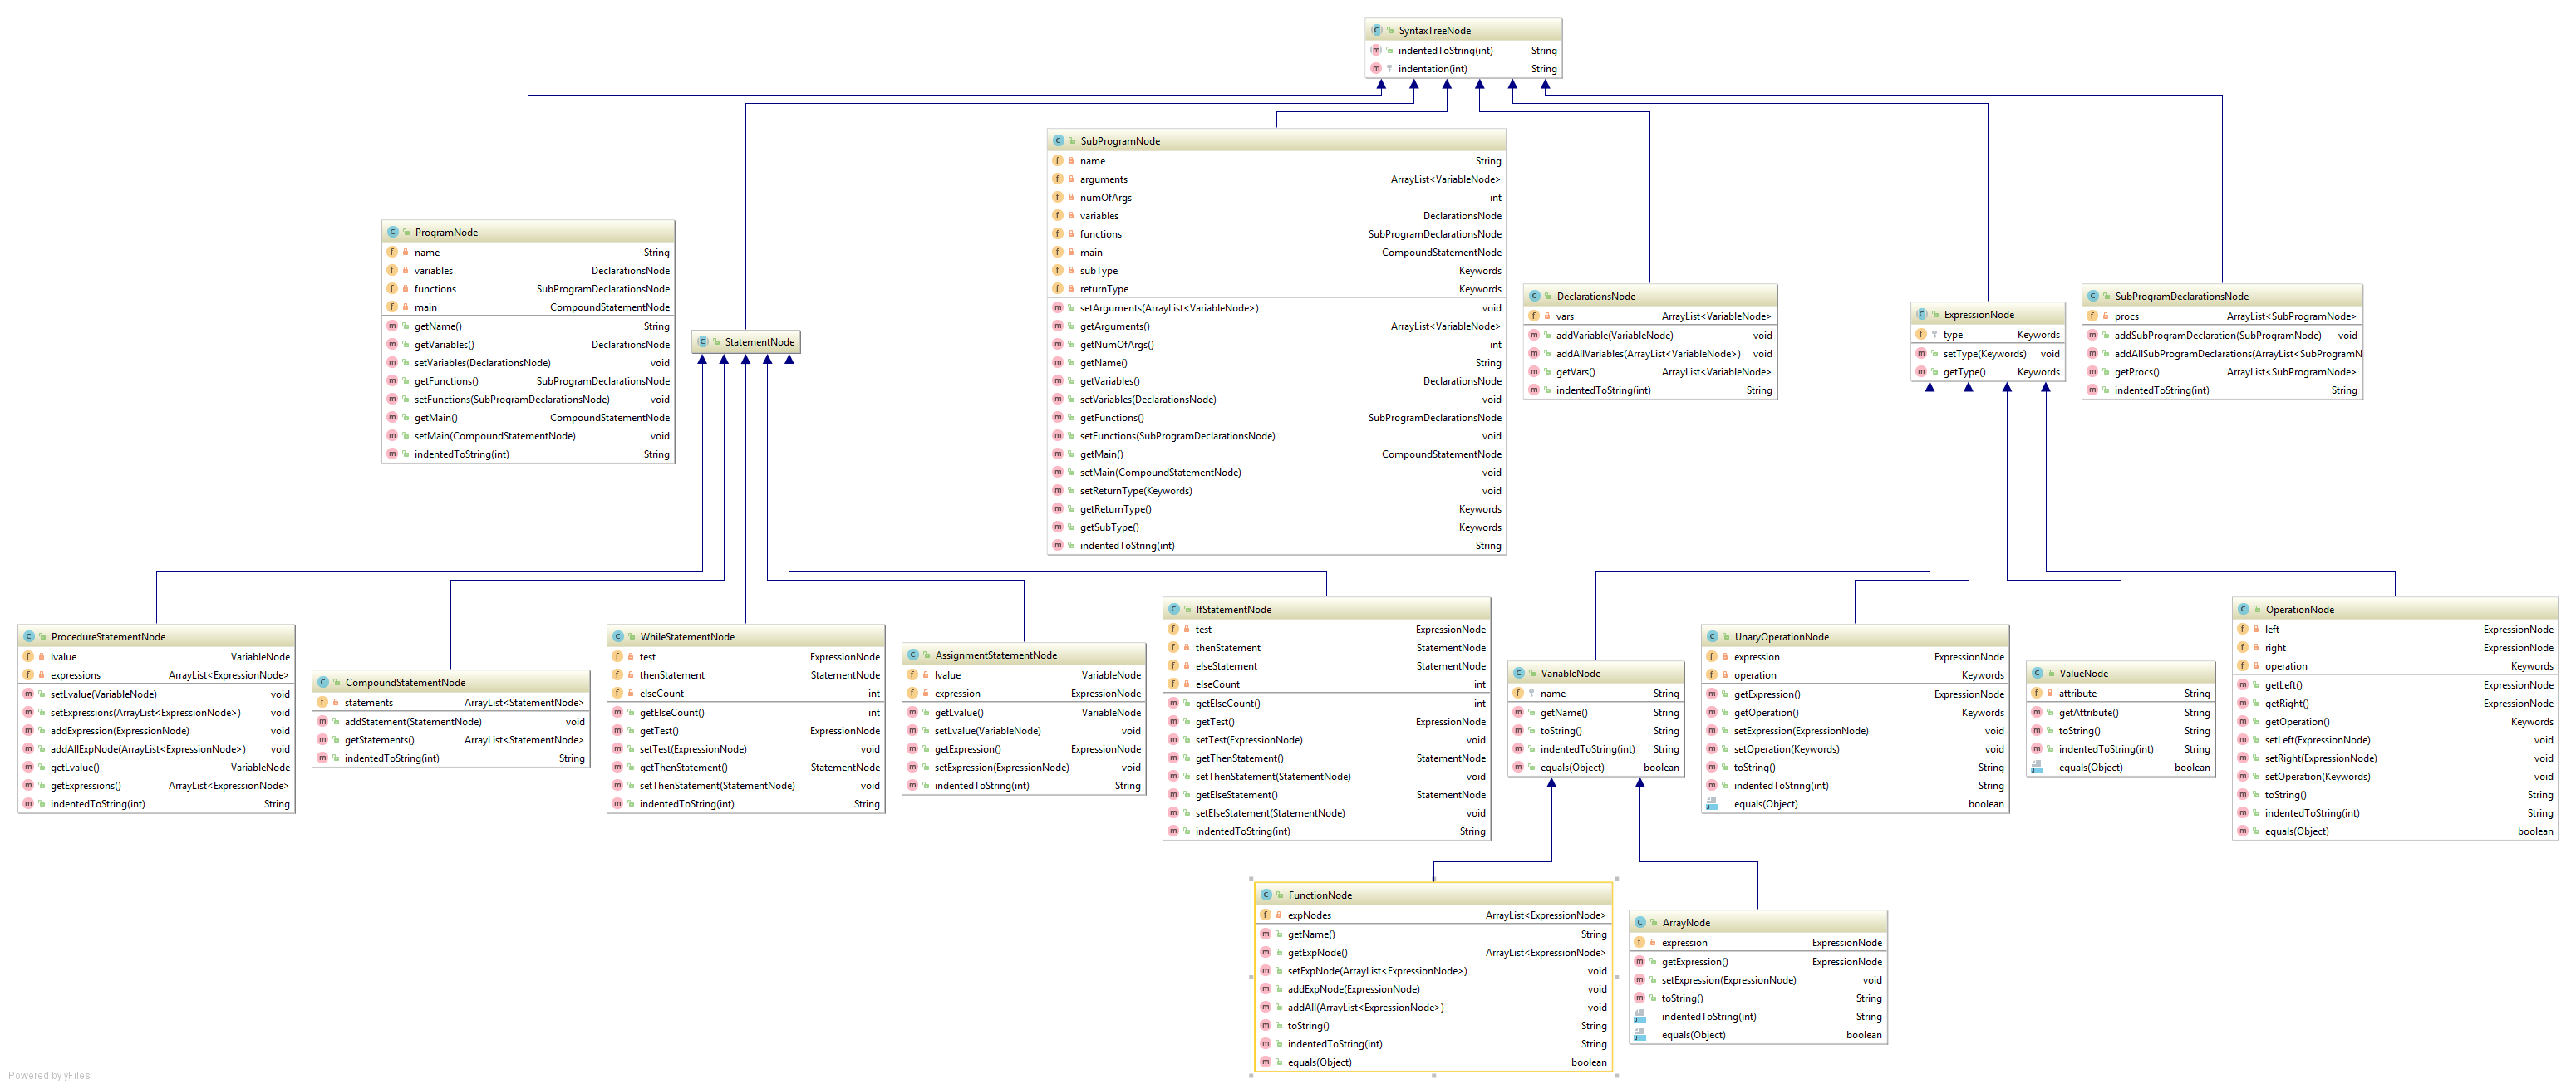
\includegraphics[width=\linewidth]{SyntaxTree.png}
	\caption{Syntax Tree Package Diagram}
\end{figure}

\section{Semantic Analyzer}
The Analyzer restructures expression nodes into their logical mathematical order and folds value nodes together as necessary.

\section{Code Generator}
The Generator produces MIPS assembly code based on the tree generated by the parser.

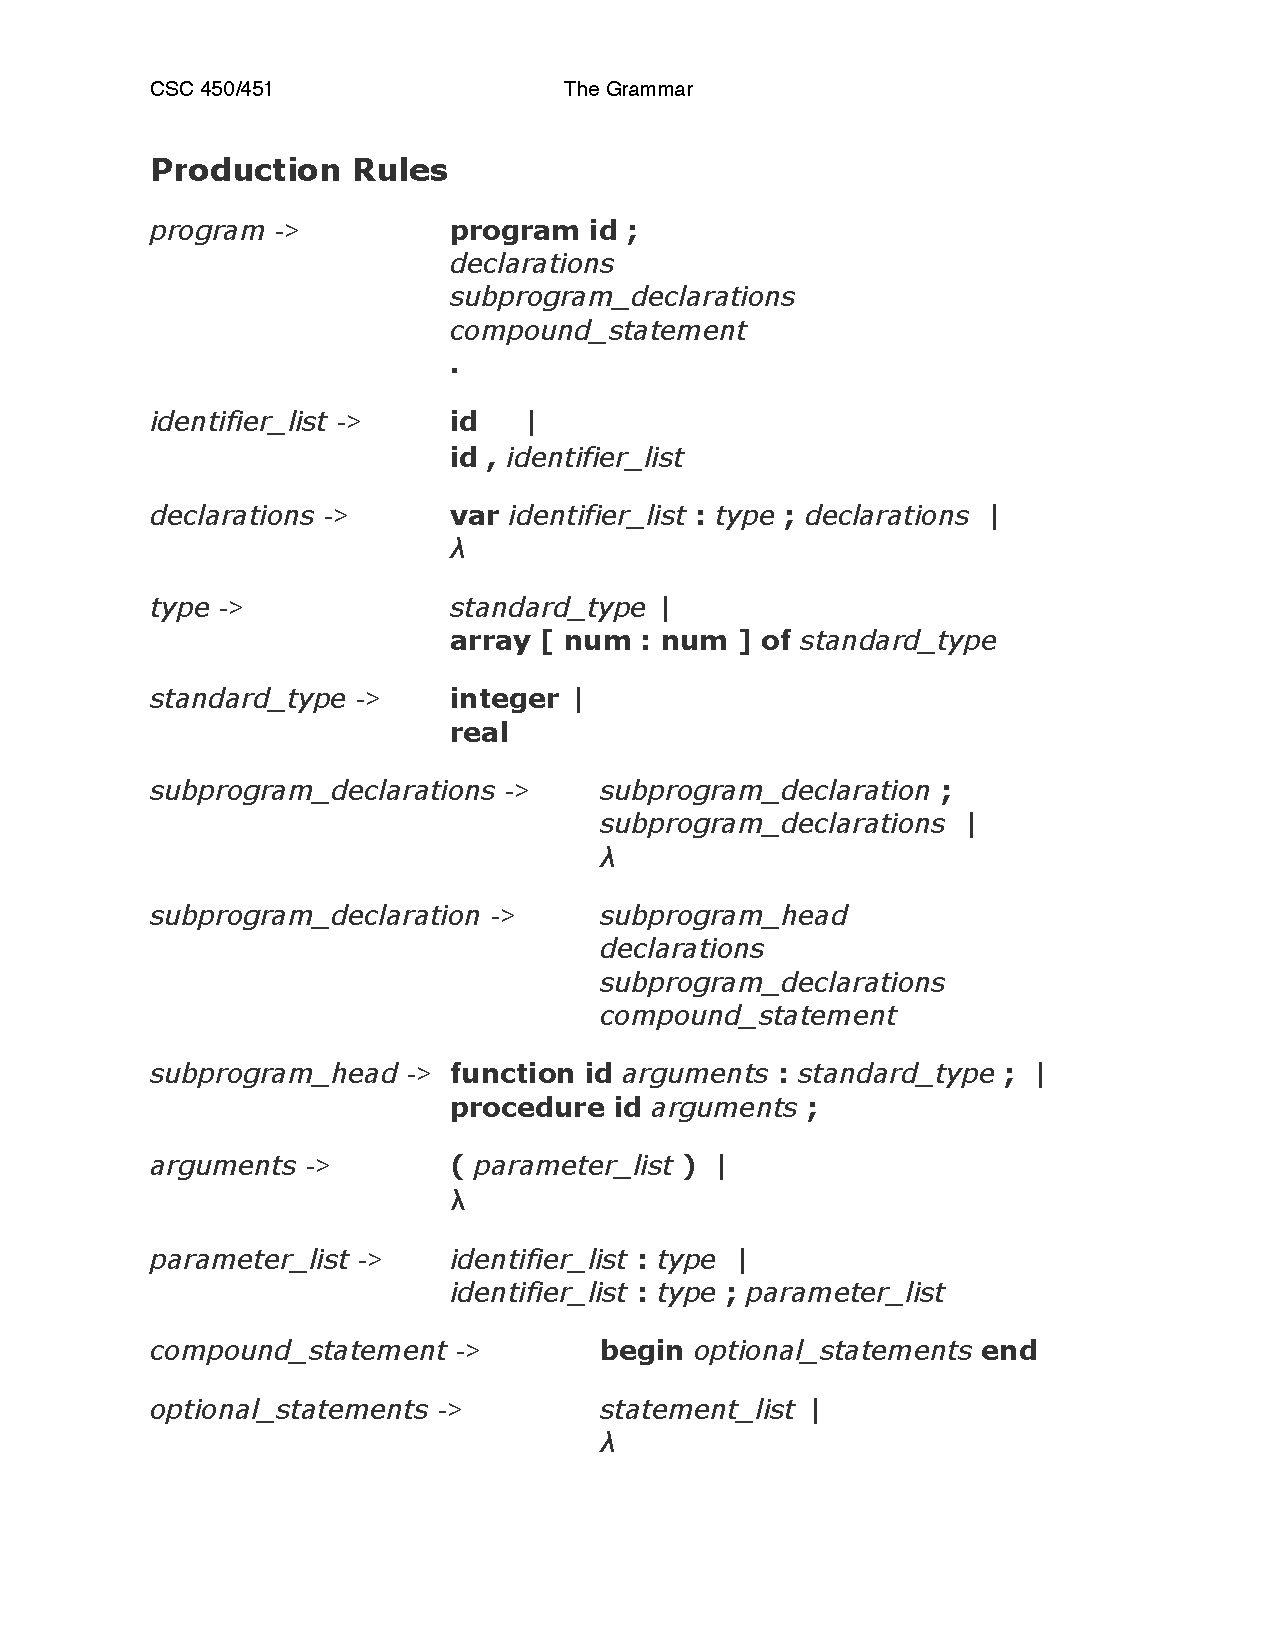
\includepdf[pages={-}]{Grammar.pdf}
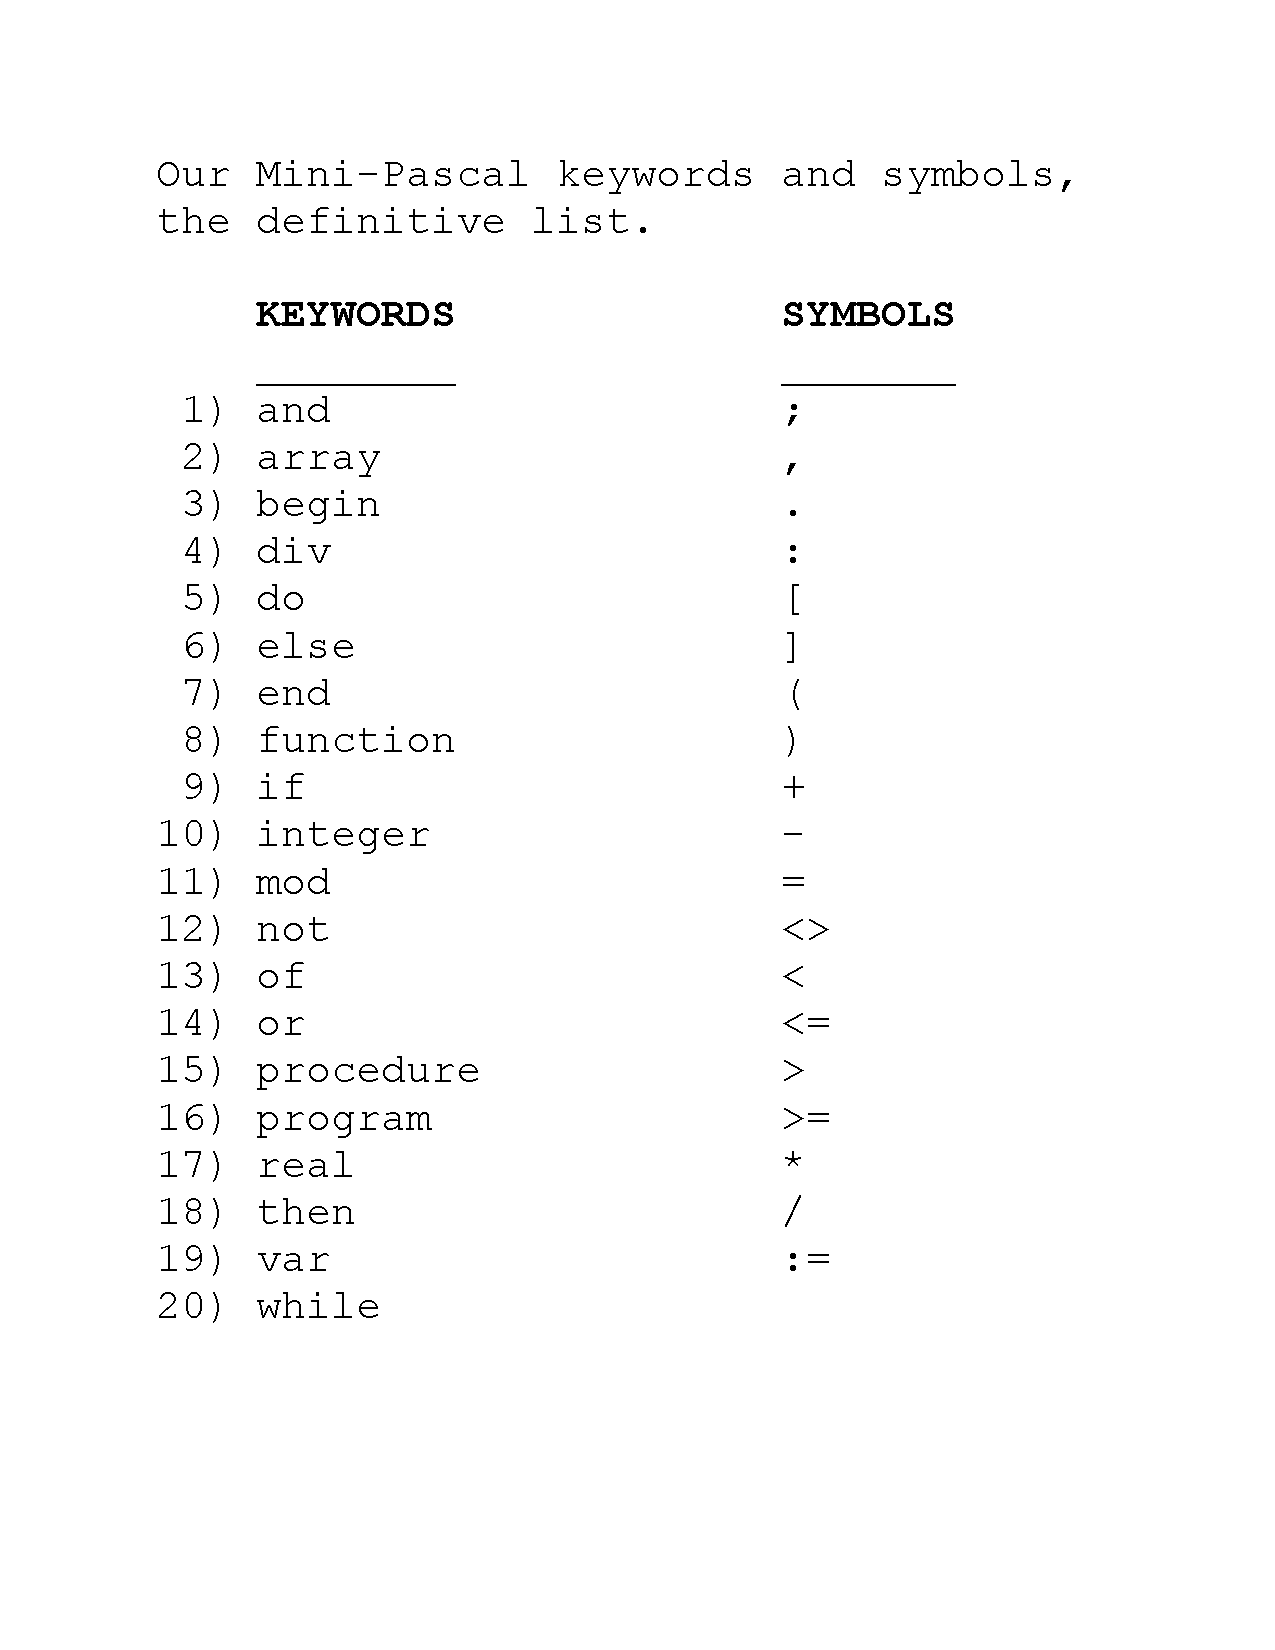
\includepdf[pages={-}]{KeywordsAndSymbols.pdf}

\end{document}

